\documentclass[journal=jctc,manuscript=article]{achemso}
\setkeys{acs}{maxauthors=0,articletitle=true}

%%%%%%%%%%%%%%%%%%%%%%%%%%%%%%%%%%%%%%%%%%

\usepackage{achemso}
\usepackage{graphics}
\usepackage{amssymb,amsfonts}
\usepackage{graphicx}
\usepackage[table]{xcolor}
\usepackage{multirow}
\usepackage{caption}
\usepackage{subcaption}
\usepackage{booktabs}
\usepackage{colortbl}
\usepackage{amsmath}
\usepackage{amsopn}
\usepackage{siunitx}
\usepackage{bm}
\usepackage{color}
\usepackage{array}
\usepackage{lscape}
\usepackage{mciteplus}
\usepackage[version=3]{mhchem}
\usepackage{ulem}
\usepackage{listings}
\usepackage{enumerate}

\SectionNumbersOn

\renewcommand{\thefootnote}{\fnsymbol{footnote}}

\newlength{\wordwidth}

\DeclareMathOperator{\tr}{Tr}

%%%%%%%%%%%%%%%%%%%%%%%%%%%%%%%%%%%%%%%%%%

\author{Janus J. Eriksen}
\email{janus.eriksen@bristol.ac.uk}
\affiliation[University of Bristol]
{School of Chemistry, University of Bristol, Cantock's Close, Bristol BS8 1TS, United Kingdom}
\author{Anders S. Christensen}
\email{anders.christensen@unibas.ch}
\affiliation[University of Basel]
{Department of Chemistry, University of Basel, Klingelbergstrasse 80, 4056 Basel, Switzerland}

%%%%%%%%%%%%%%%%%%%%%%%%%%%%%%%%%%%%%%%%%%

\title[TITLE]{Machine-Learned Decompositions of Electronic Mean-Field Energies}

%%%%%%%%%%%%%%%%%%%%%%%%%%%%%%%%%%%%%%%%%%

\begin{document}

%
%%%%%%%%%
%  ABSTRACT  %
%%%%%%%%%
%
\begin{abstract}
%

% background
% problem
% approach (techniques)
% findings
% implications
{\color{red}{Write me...}}

%
\end{abstract}
%

\newpage

%
%%%%%%%%%%%%
%   INTRODUCTION   %
%%%%%%%%%%%%
%

\section{Introduction}\label{intro_sect}

The aim of the present work is to devise a map between conventional Lewis structures, as an example of a molecular representation driven by sheer chemical intuition, and mean-field energies. As a first step, we will be concerned with Hartree-Fock energies, but we stress how the general scheme is applicable to density functional theory (DFT) as well, which constitutes a significantly more interesting use case. {\color{red}{Write me...}}

%
%%%%%%%%
%   THEORY  %
%%%%%%%%
%

\section{Theory}\label{theory_sect}

Assuming a molecular system composed of $N_{\text{nuc}}$ nuclei and $N_{\text{elec}}$ electrons spanned by an atomic orbital (AO) basis of size $N_{\text{b}}$, the Hartree-Fock functional is defined in terms of a converged 1-electron reduced density matrix (1-RDM), $\bm{D}$, as~\cite{mest}
%
\begin{align}
E_{\text{HF}}(\bm{D}) = 2\tr[\bm{h}_{\text{core}}\bm{D}] + \tr[\bm{V}_{\text{HF}}(\bm{D})\bm{D}] + h_{\text{nuc}} \ . \label{hf_energy_eq}
\end{align}
%
In Eq. \ref{hf_energy_eq}, $\bm{h}_{\text{core}}$ is the core Hamiltonian representing the kinetic energy of the electrons and their attractive interaction with the stationary nuclei of the system at hand, $h_{\text{nuc}}$ is the corresponding scalar nuclear-repulsion term, while $\bm{V}_{\text{HF}}(\bm{D})$ is the Fock potential with matrix elements
%
\begin{align}
[\bm{V}_{\text{HF}}(\bm{D})]_{\mu\nu} = \sum^{N_{\text{b}}}_{\kappa,\lambda=1}(g_{\mu\nu\kappa\lambda} - \tfrac{1}{2}g_{\mu\lambda\kappa\nu})\bm{D}_{\kappa\lambda} \label{fock_potential_eq}
\end{align}
%
in terms of Coulomb and exchange two-electron repulsion integrals in the AO basis.\\

Given the form of Eq. \ref{hf_energy_eq}, we now note how the total energy may be decomposed into a sum of contributions specific to the individual occupied molecular orbitals (MOs) of the system, of which there is a total of $N_{\text{occ}}$
%
\begin{align}
E_{\text{HF}}(\bm{D}) = \sum^{N_{\text{occ}}}_{i}(2\tr[\bm{h}_{\text{core}}\bm{D}_i] + \tr[\bm{V}_{\text{HF}}(\bm{D})\bm{D}_i]) + h_{\text{nuc}} \ . \label{orb_decomp_eq}
\end{align}
%
In Eq. \ref{orb_decomp_eq}, the individual orbital-specific 1-RDMs, $\bm{D}_i$, are defined as
%
\begin{align}
\bm{D}_i = \bm{C}_{i} \otimes \bm{C}_{i} \label{orb_spec_1rdm_eq}
\end{align}
%
where $\bm{C}_i$ denotes the $i$-th column vector of the MO coefficients matrix, $\bm{C}$, used to construct the total 1-RDM, $\bm{D}$, which is still used in Eq. \ref{orb_decomp_eq} to construct the Fock potential. In the conventional basis of canonical MOs, the orbitals themselves will be completely delocalized over the entire system. Hence, although the linear combinations of AOs that define the individual MOs may be symmetry adapted, one cannot in general expect any degree of systematic grouping of the individual contributions to the decomposition in Eq. \ref{orb_decomp_eq}. In the lack of any repeating patterns among the MO contributions, the hope of addressing the overall problem, that is, the mapping of chemical bonds to total electronic energies, remains intractable.\\

%
\begin{figure}[ht]
\begin{center}
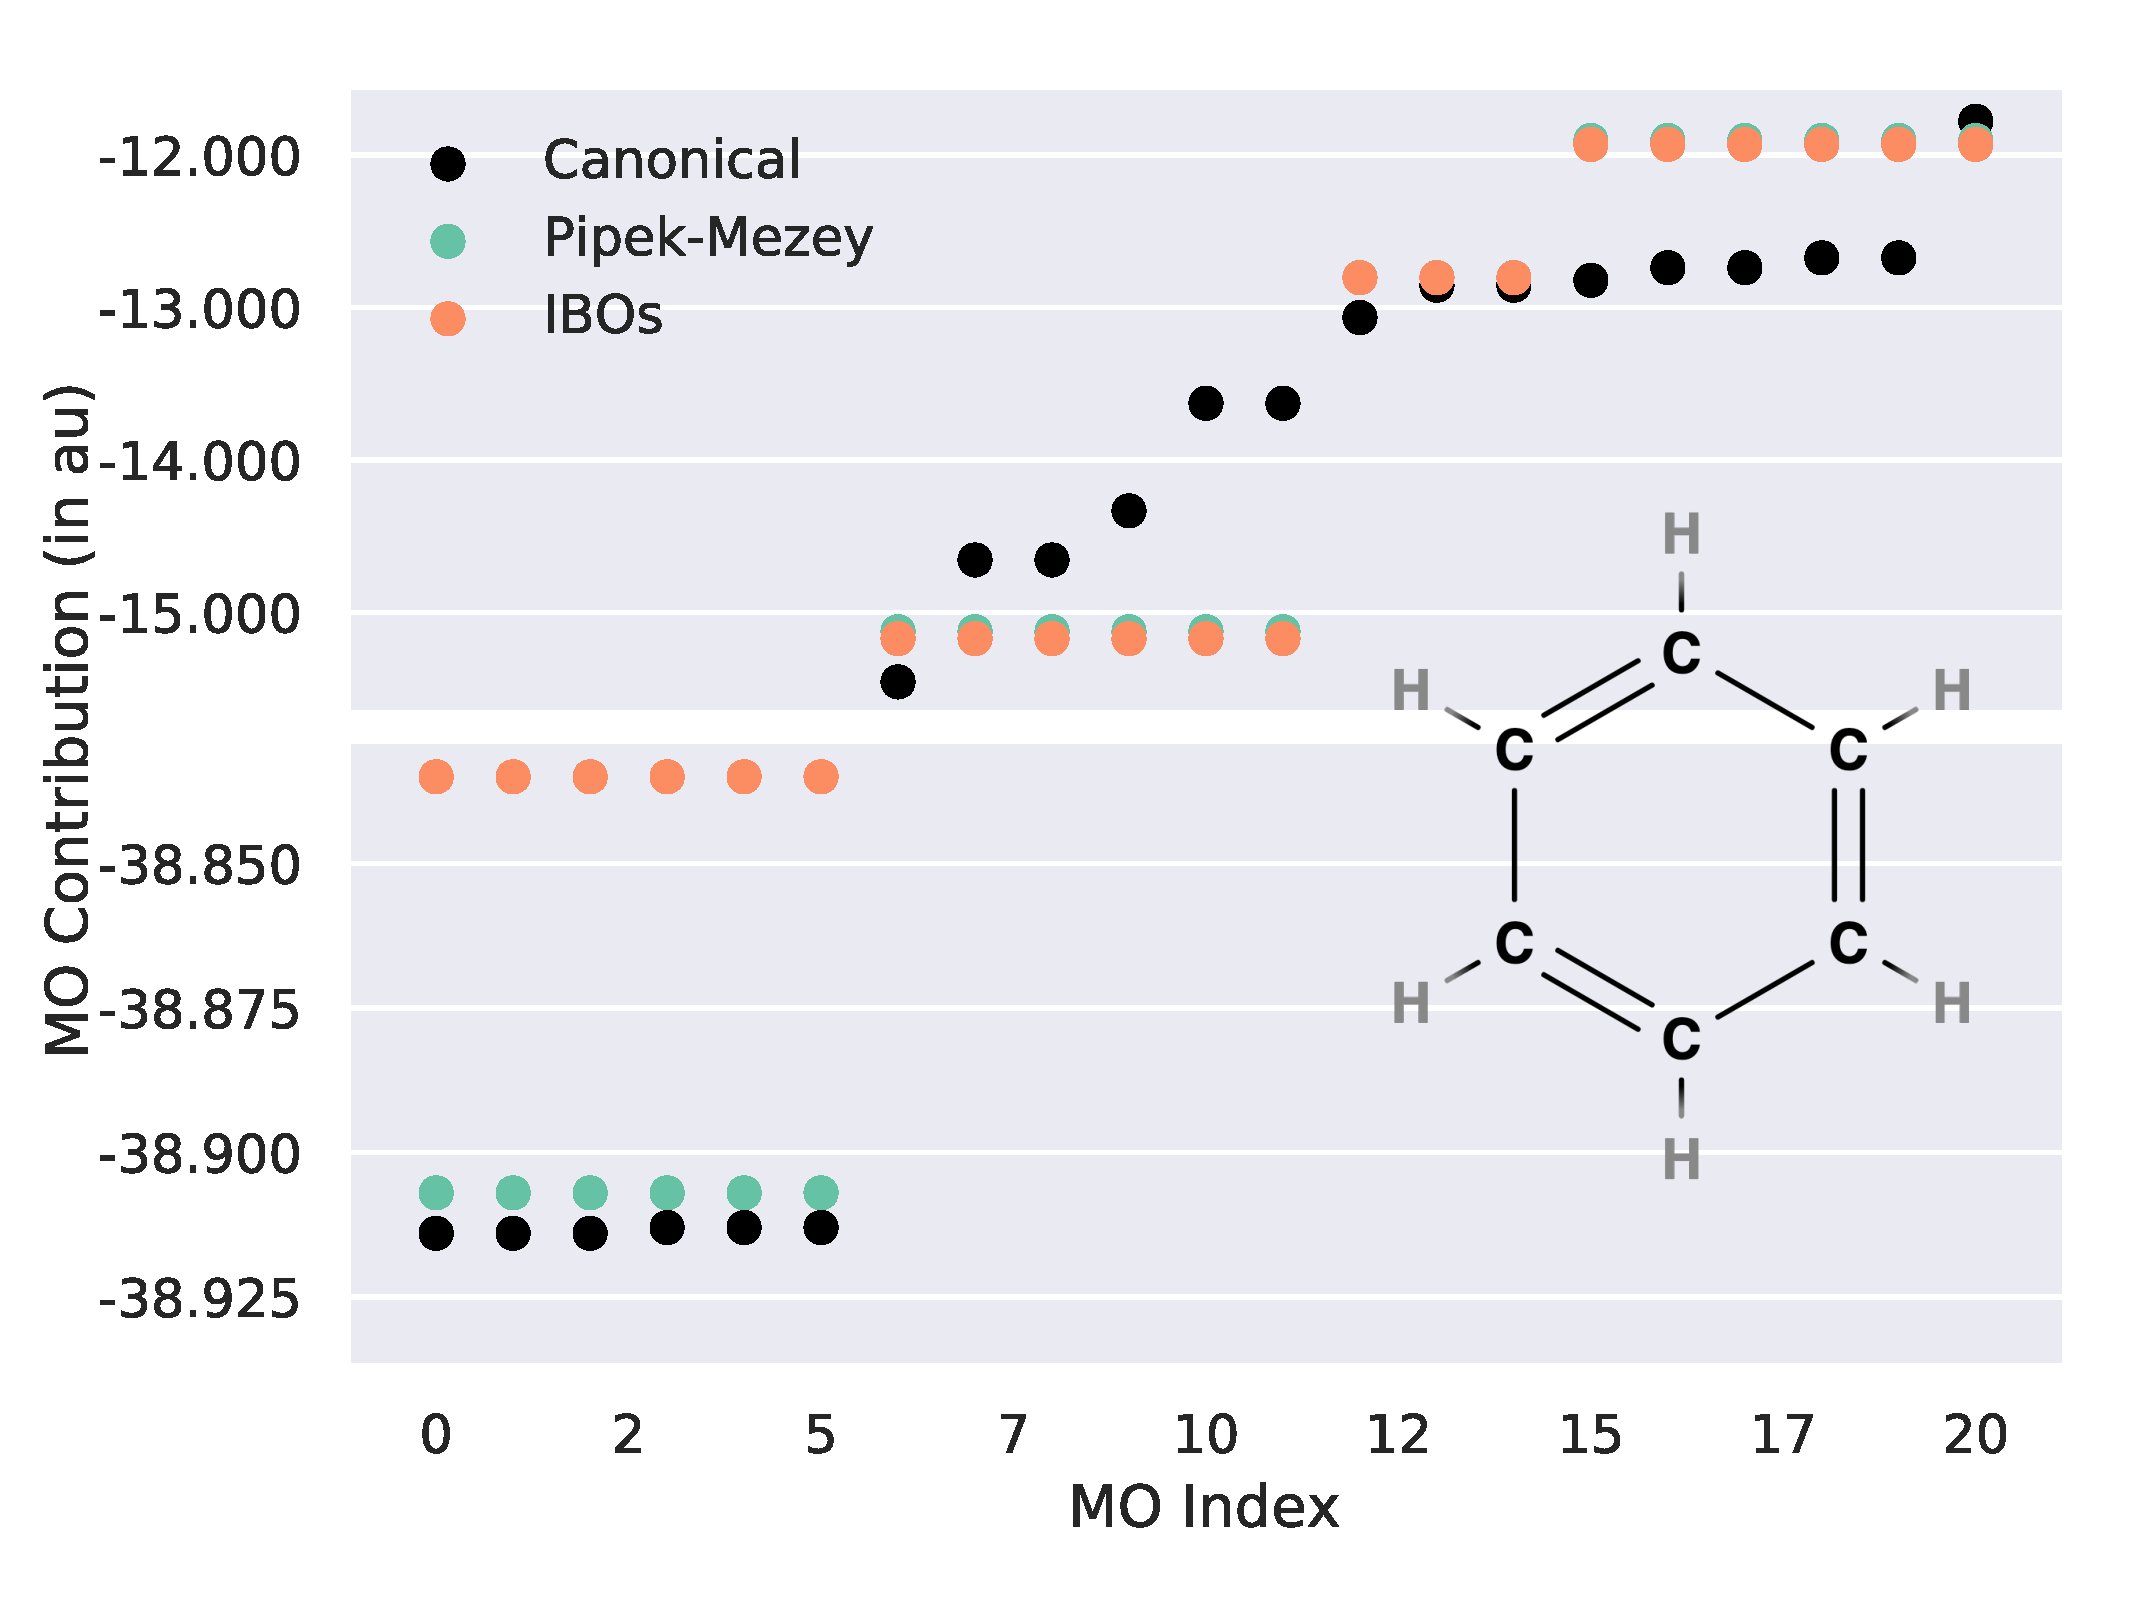
\includegraphics[width=\textwidth]{figures/c6h6_hf_2.pdf}
\caption{Orbital-specific contributions to the total HF/6--31G energy of benzene using $D_{2\text{h}}$ point-group symmetry and either canonical RHF or Pipek-Mezey localized MOs.}
\label{c6h6_hf_fig}
\end{center}
\end{figure}
%
As an illustration of this point, Figure \ref{c6h6_hf_fig} shows the distribution of each of the contributions from the 21 occupied MOs of the benzene molecule. As is evident from Figure \ref{c6h6_hf_fig}, the energy contributions are generally non-degenerate despite the high symmetry of the molecule. However, while the total HF energy and hence the total 1-RDM are invariant under rotations of the occupied MOs, the orbital-specific 1-RDMs in Eq. \ref{orb_spec_1rdm_eq} are not. That is, one is free to perform a unitary transformation of the original set of canonical occupied MOs into some updated basis and repeat the decomposition in Eq. \ref{orb_decomp_eq}. As an obvious option, one may choose to apply any of a number of localizaiton procedures to the problem. However, regardless of how local (in a spatial sense) the transformed MOs may be, if these fail to preserve the traits present in Lewis structure representations of the molecule, such as, e.g., $\sigma$- and $\pi$-symmetries in planar systems, their use in the present context will be not mark an improvement over canonical MOs. On the other hand, if the localization procedure preserves such symmetries and bond patterns, it can indeed offer a notable improvement over canonical MOs. This is depicted in Figure \ref{c6h6_hf_fig} through results obtained using Pipek-Mezey localized MOs~\cite{pipek_mezey_jcp_1989}.\\

From the Pipek-Mezey results in Figure \ref{c6h6_hf_fig}, we clear see a correlation between what is to be expected on the basis of the Lewis structure representation of benzene and what the decomposition in Eq. \ref{orb_decomp_eq} returns. Given the high symmetry (full point group: $D_{6\text{h}}$, computational subgroup: $D_{2\text{h}}$), the 6 core orbitals of the carbons are indistinguishable, as are the 6 C--C bonds and the 6 C--H bonds. The decomposition even yields contributions from 3 degenerate carbon double bonds, in perfect agreement with the conventional Kekul{\'e} formula in Figure \ref{c6h6_hf_fig}. Neither of these features are present in the decomposition based on canonical MOs, except for the core orbitals; however, not even these are degenerate. In order to further illustrate the potential of the proposed decomposition, Figure \ref{c10h8_hf_fig} shows a comparison between the benzene decomposition in terms of Pipek-Mezey MOs of Figure \ref{c6h6_hf_fig} and the corresponding decomposition for the related naphthalene molecule.\\
%
\begin{figure}[ht]
\begin{center}
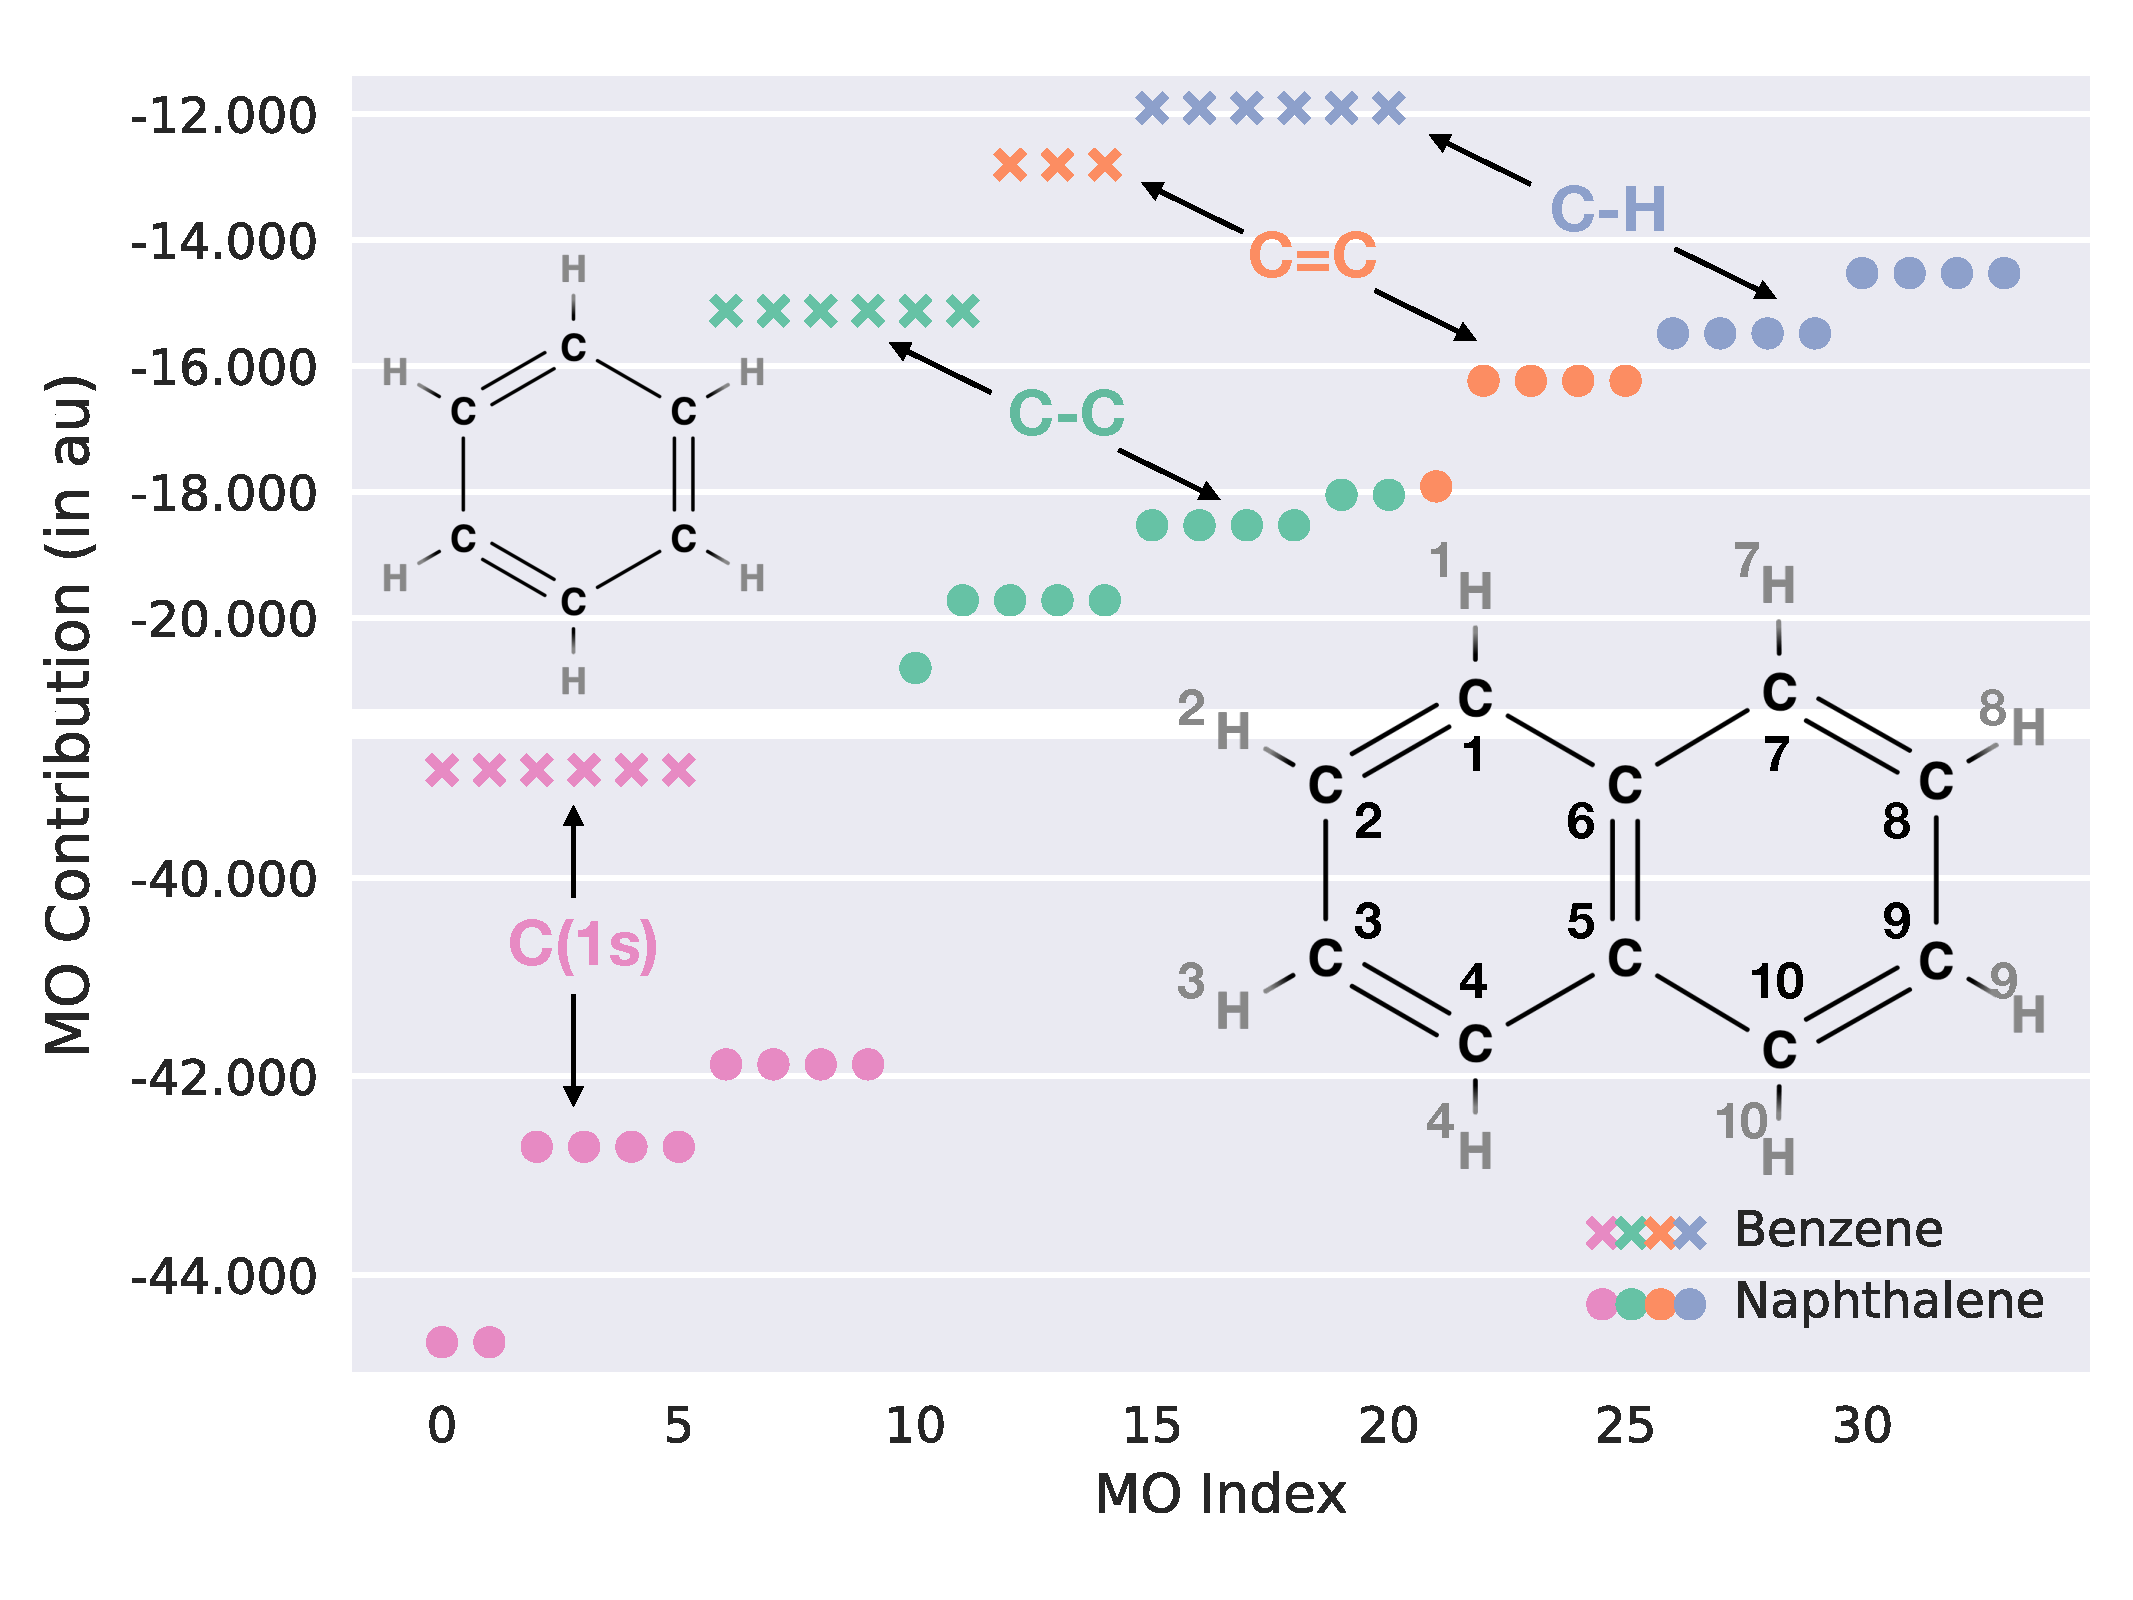
\includegraphics[width=\textwidth]{figures/c10h8_hf_2.pdf}
\caption{Comparison of the orbital-specific contributions to the total HF/6--31G energies of benzene and naphthalene using $D_{2\text{h}}$ point-group symmetry and Pipek-Mezey localized MOs.}
\label{c10h8_hf_fig}
\end{center}
\end{figure}
%

In comparison with the previous benzene example, naphthalene has a much reduced symmetry ($D_{2\text{h}}$ point group). As such, the contributions to the naphthalene decomposition appear much less ordered at a first glance, but upon assigning the localized MOs to single and pairs of atomic centers, the mapping the the Kekul{\'e} representation shown in Figure \ref{c10h8_hf_fig} is restored. In Table \ref{c10h8_hf_table}, the magnitudes of the different degenerate contributions are compared for the naphthalene case and their sum is shown to equal the correct value of $E_{\text{HF}} - h_{\text{nuc}} = -840.51136$ au.
%
\begin{table}[ht]
\begin{center}
\begin{tabular}{l|cccc|r}
\toprule
\multicolumn{1}{c|}{Type} & \multicolumn{1}{c}{Component} & \multicolumn{1}{c}{Component} & \multicolumn{1}{c}{Component} & \multicolumn{1}{c|}{Component} & \multicolumn{1}{c}{Energy} \\
\midrule\midrule
C$-$H & C2 \& H2 & C3 \& H3 & C8 \& H8 & C9 \& H9 & $-14.527$ \\
C$-$H & C1 \& H1 & C4 \& H4 & C7 \& H7 & C10 \& H10 & $-15.484$ \\
C$=$C & C1 \& C2 & C3 \& C4 & C7 \& C8 & C9 \& C10 & $-16.236$ \\
C$=$C & C5 \& C6 & & & & $-17.913$ \\
C$-$C & C2 \& C3 & C8 \& C9 & & & $-18.047$ \\
C$-$C & C1 \& C2 & C3 \& C4 & C7 \& C8 & C9 \& C10 & $-18.531$ \\
C$-$C & C1 \& C6 & C4 \& C5 & C6 \& C7 & C5 \& C10 & $-19.722$ \\
C$-$C & C5 \& C6 & & & & $-20.796$ \\
C(1s) & C2 & C3 & C8 & C9 & $-41.879$ \\
C(1s) & C1 & C4 & C7 & C10 & $-42.709$ \\
C(1s) & C5 & C6 & & & $-44.678$ \\
\bottomrule
\end{tabular}
\end{center}
\caption{Energy contributions per component (in au) to the total HF/6--31G energy of naphthalene using $D_{2\text{h}}$ point-group symmetry and Pipek-Mezey localized MOs (cf. Figure \ref{c10h8_hf_fig} for atom labels). The total sum equals $-840.51136$ au, which, upon adding the nuclear-repulsion term $h_{\text{nuc}} = +457.29068$ au, results in $E_{\text{HF}} = -383.22068$ au.}
\label{c10h8_hf_table}
\end{table}
%

%
%%%%%%%%%%%
%  COMP DETAILS %
%%%%%%%%%%%
%

\section{Computational Details}\label{comp_details_sect}

{\color{red}{Write me...}}

%
%%%%%%%%
% RESULTS  %
%%%%%%%%
%

\section{Results}\label{results_sect}

\begin{itemize}
\item Train on series of polyaromatic hydrocarbons (arenes), predict their total energies afterwards.
\item Train on series of linear aliphatic hydrocarbons, predict their total energies afterwards.
\item Train on both series of molecules, predict all total energies afterwards.
\end{itemize}

%
%%%%%%%%%%
% CONCLUSION %
%%%%%%%%%%
%

\section{Conclusion and Summary}\label{conclusion_sect}

%
%%%%%%%%%%%%%%
%  ACKNOWLEDGMENT  %
%%%%%%%%%%%%%%
%
\section*{Acknowledgments}
%

J. J. E. is grateful to Prof. Frederick R. Manby of the University of Bristol in his role as host and for various insightful discussions related to the present work. J. J. E. is further grateful to the Independent Research Fund Denmark for financial support.

\newpage

\bibliography{/Users/janusje/Dropbox/refs.bib}

\end{document}